\section{Visualisations}
This section provides the visual synthesis Scopus Q1 reviewers expect: the PRISMA flow (Fig.~\ref{fig:prisma}), publication trend (Fig.~\ref{fig:trend}), dataset popularity (Fig.~\ref{fig:dspop}), the field taxonomy (Fig.~\ref{fig:tax}), and the deployment pipeline (Fig.~\ref{fig:pipe}).

\begin{figure}[t]\centering
\resizebox{\columnwidth}{!}{%
\begin{tikzpicture}[font=\scriptsize,node distance=4mm,
 b/.style={draw,rounded corners,fill=blue!8,text width=5.8cm,align=center,minimum height=5mm}]
\node[b](a){Records identified ($\sim$220)};
\node[b,below=of a](c){After de-duplication (140)};
\node[b,below=of c](d){Title/abstract screened (95)};
\node[b,below=of d](e){Full-text assessed (64)};
\node[b,below=of e,fill=green!12](f){\textbf{Included in synthesis (50)}};
\draw[-{Stealth}](a)--(c);\draw[-{Stealth}](c)--(d);\draw[-{Stealth}](d)--(e);\draw[-{Stealth}](e)--(f);
\end{tikzpicture}
}
\caption{PRISMA-style selection flow.}\label{fig:prisma}\end{figure}

\begin{figure}[t]\centering
\resizebox{\columnwidth}{!}{%
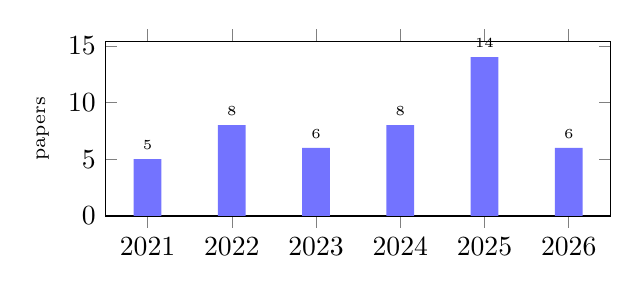
\begin{tikzpicture}\begin{axis}[width=8cm,height=3.8cm,ybar,bar width=10pt,
 symbolic x coords={2021,2022,2023,2024,2025,2026},xtick=data,
 ymin=0,ylabel={\scriptsize papers},nodes near coords,every node near coord/.append style={font=\tiny}]
\addplot[fill=blue!55,draw=none] coordinates {(2021,5)(2022,8)(2023,6)(2024,8)(2025,14)(2026,6)};
\end{axis}\end{tikzpicture}
}
\caption{Publication trend, 2021--2026 (the 2026 count is partial-year).}\label{fig:trend}\end{figure}

\begin{figure}[t]\centering
\resizebox{\columnwidth}{!}{%
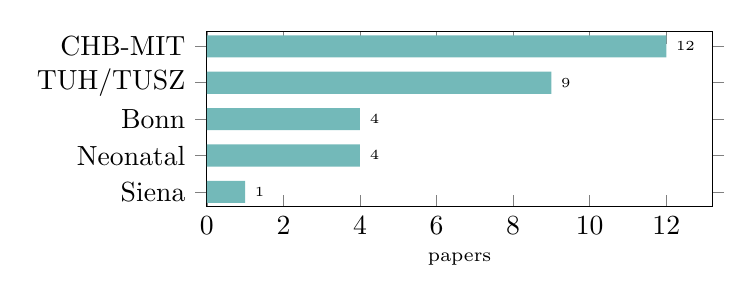
\begin{tikzpicture}\begin{axis}[width=8cm,height=3.8cm,xbar,bar width=8pt,
 symbolic y coords={Siena,Neonatal,Bonn,TUH/TUSZ,CHB-MIT},ytick=data,
 xmin=0,xlabel={\scriptsize papers},nodes near coords,every node near coord/.append style={font=\tiny}]
\addplot[fill=teal!55,draw=none] coordinates {(1,Siena)(4,Neonatal)(4,Bonn)(9,TUH/TUSZ)(12,CHB-MIT)};
\end{axis}\end{tikzpicture}
}
\caption{Dataset popularity across the corpus.}\label{fig:dspop}\end{figure}

\begin{figure}[t]\centering
\resizebox{\columnwidth}{!}{%
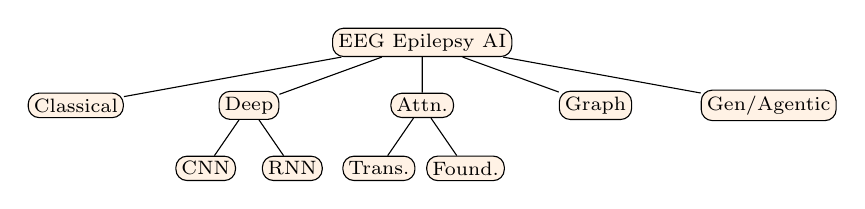
\begin{tikzpicture}[font=\scriptsize,level distance=8mm,
 every node/.style={draw,rounded corners,fill=orange!10,inner sep=2pt},
 level 1/.style={sibling distance=22mm},level 2/.style={sibling distance=11mm}]
\node{EEG Epilepsy AI}
 child{node{Classical}}
 child{node{Deep}
  child{node{CNN}}
  child{node{RNN}}}
 child{node{Attn.}
  child{node{Trans.}}
  child{node{Found.}}}
 child{node{Graph}}
 child{node{Gen/Agentic}};
\end{tikzpicture}
}
\caption{Architecture taxonomy of the field.}\label{fig:tax}\end{figure}

\begin{figure}[t]\centering
\resizebox{\columnwidth}{!}{%
\begin{tikzpicture}[font=\tiny,node distance=2.0mm,
 s/.style={draw,fill=gray!10,rounded corners,text width=1.55cm,align=center,minimum height=4mm}]
\node[s](p){Patient + wearable};
\node[s,right=of p](g){Gateway/Cloud};
\node[s,right=of g](pre){Preprocess + features};
\node[s,below=of pre](m){AI model};
\node[s,left=of m](x){XAI + governance};
\node[s,left=of x](v){Clinician + EMR};
\draw[-{Stealth}](p)--(g);\draw[-{Stealth}](g)--(pre);\draw[-{Stealth}](pre)--(m);
\draw[-{Stealth}](m)--(x);\draw[-{Stealth}](x)--(v);\draw[-{Stealth}](v.south)to[out=-90,in=-90](p.south);
\end{tikzpicture}
}
\caption{Healthcare deployment pipeline with feedback loop.}\label{fig:pipe}\end{figure}
